Исследуемый сценарий --- известна криптограмма и неизвестен
ни алгоритм шифрования, ни
алгоритм шифрования, необходимо получить исходный открытый
текст. В этой части описан примерный алгоритм идентификации 
шифра.

Для него понадобится следующая классификация шифров:

\begin{enumerate}
\item \textbf{Перестановочные шифры} --- шифр с фиксированным периодом 
    $n$ подразумевает разбиение исходного текста на блоки по 
    n символов и использование для каждого такого блока некоторой 
    перестановки $E$. Ключом такого шифра является используемая 
    при шифровании перестановочная матрица $P$ или вектор $t$, указывающий 
    правило перестановки. Таким образом, общее число возможных 
    ключей определяется длиной блока $n$ и равно $n!$. При дешифрации 
    используется матрица обратной перестановки D, являющаяся 
    обратной к матрице $P$ по умножению, то есть $D \times P = I$, 
    где $I$ — единичная матрица;
\item \textbf{Моноалфавитные шифры} --- шифры, в которых каждой букве 
    кодируемого текста ставится в соответствие однозначно какая-то
    шифрованная буква;
\item \textbf{Полиалфавитные шифры} --- шифры, в которых каждой букве 
    Суть полиалфавитного шифра заключается в циклическом применении 
    нескольких моноалфавитных шифров к определенному числу букв 
    шифруемого текста. Например, пусть у нас имеется некоторое 
    сообщение $x_1, x_2, x_3, \dots, x_n, \dots, x_{2n}, \dots$ 
    которое надо 
    зашифровать. При использовании полиалфавитного шифра имеется 
    несколько моноалфавитных шифров (например, n штук).
    Самым важным эффектом, достигаемым при использовании 
    полиалфавитного шифра, является маскировка частот появления 
    тех или иных букв в тексте, на основании которой обычно очень 
    легко вскрываются моноалфавитные шифры;
\item \textbf{Смешанные шифры} --- шифры, в которых сочетаются 
    свойства перечисленных выше шифров.
\end{enumerate}

Каждая из этих категорий оставляет после шифрования статистический 
отпечаток, который возможно заметить с помощью описываемых 
далее методов. Для их работы необходимо 1000 или более 
знаков шифротекста.

Возможно выяснить границу между шифрами перестановки 
и всеми остальными, сравнив встечаемость символов в шифротексте 
и в натуральных языках. Если шифр перестановочный, его частотная 
характеристика совпадет с характеристикой какого-либо из языков.

Следующий шаг --- определение моноалфавитного шифра. 
Для этого можно посчитать индекс совпадений. Если он будет в районе
0.06, то можно заключить, что это шифр моноалфавитной подстановки.
Если он меньше, то это либо полиалфавитная подстановка, либо 
смешанный шифр.

Дальнейший анализ построен на основе следующих величин:

\begin{enumerate}
\item \textbf{IC} --- индекс совпадения умноженный на 1000;
\item \textbf{MIC} --- максимальный индекс совпадения для периодов
    с 1 по 15 умноженный на 1000;
\item \textbf{DIC} --- индекс совпадения биграмм
    умноженный на 10000;
\item \textbf{EDI} --- индекс совпадения биграмм для четных по порядку пар
    умноженный на 10000;
\item \textbf{LR} --- квадратный корень от процента от 3 повторений 
    символа умноженный на 1000;
\item \textbf{ROD} --- отношение повторений на нечетном интервале ко
    всем отношениям в тексте.
\item \textbf{DIC} --- индекс совпадения биграмм
    умноженный на 10000;
\item \textbf{SDD} --- средняя величина дисперсии букв в биграммах.
\end{enumerate}

С их помощью можно составить таблицы, характеризующие шифры 
сложнее моноалфавитных подстановок. Такие таблицы были постоены
и опубликованы Американским Сообществом Криптоаналитиков.
Выписки из таблиц приведены в рисунках 
\ref{aca-table1} и \ref{aca-table2}.

Величины для изучаемых шифров использованы в фреймворке,
при достаточном объеме шифротекста они позоляют определить
использованный шифр.

\begin{figure}[h]
\noindent\centering{
    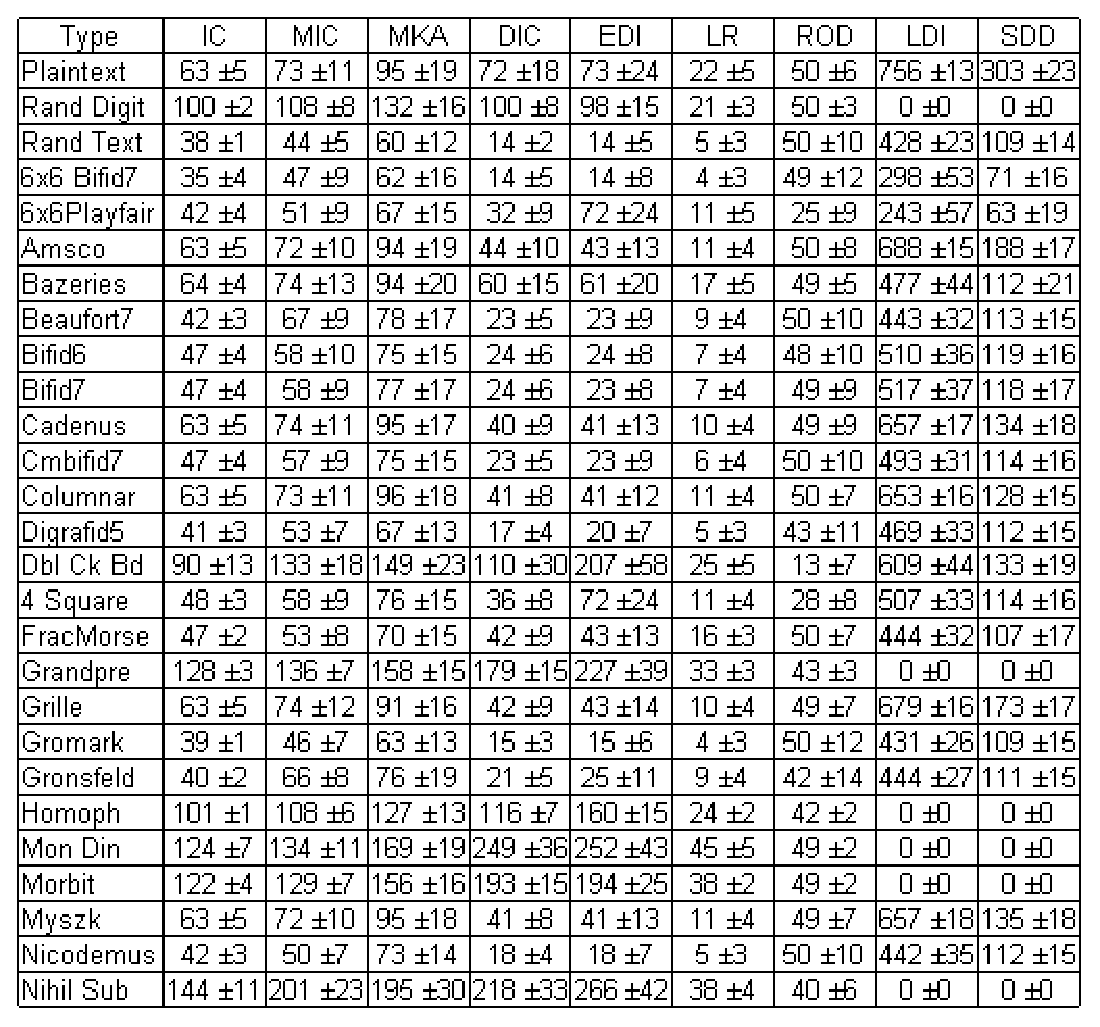
\includegraphics[width=95mm]{\globalImages/aca-table1.eps}
}
\caption{Таблица ACA характеристик полиалфавитных шифров}
\label{aca-table1}
\end{figure}

\begin{figure}[h]
\noindent\centering{
    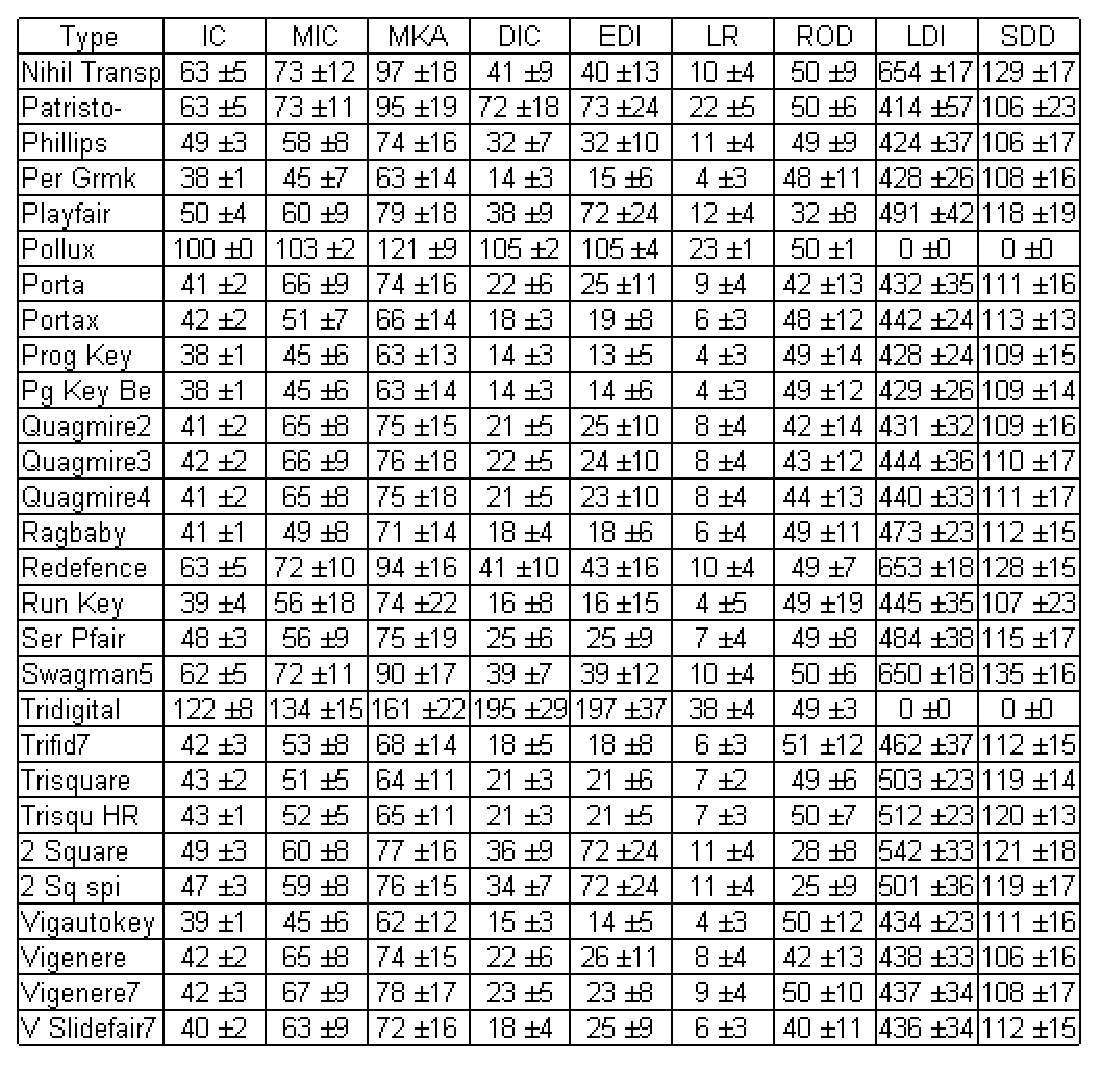
\includegraphics[width=95mm]{\globalImages/aca-table2.eps}
}
\caption{Таблица ACA характеристик полиалфавитных шифров}
\label{aca-table2}
\end{figure}
